\documentclass{standalone}

\usepackage{tikz}
\usetikzlibrary{arrows.meta, positioning, calc}

\begin{document}
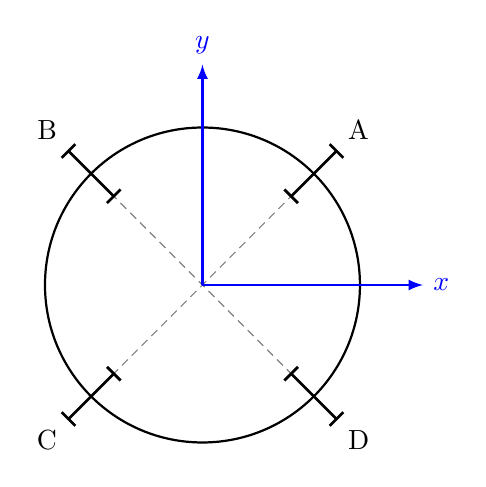
\begin{tikzpicture}[>=latex]

\pgfmathsetmacro{\r}{2}
\pgfmathsetmacro{\dr}{0.8}

\coordinate (O) at (0, 0);
\coordinate (A) at ({\r*cos(45)},     {\r*sin(45)});
\coordinate (B) at ({\r*cos(45+90)},  {\r*sin(45+90});
\coordinate (C) at ({\r*cos(45+180)}, {\r*sin(45+180)});
\coordinate (D) at ({\r*cos(45+270)}, {\r*sin(45+270)});
\coordinate (Sp) at (0.2, 0.2);
\coordinate (Sm) at (-0.2, -0.2);

\draw[gray, densely dashed, line width=0.4pt] (A) -- (C);
\draw[gray, densely dashed, line width=0.4pt] (B) -- (D);

\draw[black, thick] (O) circle (\r);

\draw[thick, blue, ->] (0,0) -- (\r+\dr, 0) node[right] {$x$};
\draw[thick, blue, ->] (0,0) -- (0, \r+\dr) node[above] {$y$};

\pgfmathsetmacro{\ds}{0.3}
\coordinate (mA) at ($(A) + (-\ds, -\ds)$);
\coordinate (pA) at ($(A) + (\ds, \ds)$);
\draw[|-|, line width=1pt] (mA) -- (pA) node[above right] {A}; 

\coordinate (mB) at ($(B) + (\ds, -\ds)$);
\coordinate (pB) at ($(B) + (-\ds, \ds)$);
\draw[|-|, line width=1pt] (mB) -- (pB) node[above left] {B}; 

\coordinate (mC) at ($(C) + (\ds, \ds)$);
\coordinate (pC) at ($(C) + (-\ds, -\ds)$);
\draw[|-|, line width=1pt] (mC) -- (pC) node[below left] {C}; 

\coordinate (mD) at ($(D) + (-\ds, \ds)$);
\coordinate (pD) at ($(D) + (\ds, -\ds)$);
\draw[|-|, line width=1pt] (mD) -- (pD) node[below right] {D}; 

\end{tikzpicture}
\end{document}
